\section{MCMC Sampling Algorithm for QVP}\label{sec:mcmc}
%
The priors outlined above results in known conditional posterior distributions and therefore an efficient Gibbs sampling scheme which iterates through the following updates:
\begin{enumerate}
    \item $\boldsymbol{\beta}^{(s)} \sim p(\boldsymbol{\beta}\mid \boldsymbol{y},\boldsymbol{\Sigma}^{(s-1)},\beta_0^{(s-1)},\boldsymbol{\alpha}^{(s-1)},\boldsymbol{\mu}^{(s-1)},\boldsymbol{\Omega}^{(s-1)} )$,
    \item $\boldsymbol{\Sigma}^{(s)} \sim p(\boldsymbol{\Sigma}\mid \boldsymbol{y},\boldsymbol{\beta}^{(s)},\beta_0^{(s-1)},\boldsymbol{\alpha}^{(s-1)},\boldsymbol{\mu}^{(s-1)}, \boldsymbol{\Omega}^{(s-1)})$, 
    \item $\beta_0^{(s)} \sim p(\beta_0\mid \boldsymbol{y},\boldsymbol{\beta}^{(s)},\boldsymbol{\Sigma}^{(s)},\boldsymbol{\alpha}^{(s-1)},\boldsymbol{\mu}^{(s-1)},\boldsymbol{\Omega}^{(s-1)} )$, 
    \item $\boldsymbol{\alpha}^{(s)} \sim p(\boldsymbol{\alpha} \mid \boldsymbol{y},\boldsymbol{\beta}^{(s)},\boldsymbol{\Sigma}^{(s)},\beta_0^{(s)},\boldsymbol{\mu}^{(s-1)},\boldsymbol{\Omega}^{(s-1)} )$, 
    \item $\boldsymbol{\mu}^{(s)} \sim p(\boldsymbol{\mu} \mid \boldsymbol{y},\boldsymbol{\beta}^{(s)},\boldsymbol{\Sigma}^{(s)},\beta_0^{(s)},\boldsymbol{\alpha}^{(s),},\boldsymbol{\Omega}^{(s-1)})$, 
    \item $\boldsymbol{\Omega}^{(s)} \sim p(\Omega\mid \boldsymbol{y},\boldsymbol{\beta}^{(s)},\boldsymbol{\Sigma}^{(s)},\beta_0^{(s)},\boldsymbol{\alpha}^{(s)},\boldsymbol{\mu}^{(s)} )$, ,
\end{enumerate}
%
for $s = (1,\dotsc,S)$ until convergence. The conditional posteriors are given in Appendix~\ref{app:qvp-posteriors}.
%
The main computational bottleneck in sampling from Posterior~\ref{eq:Posterior_beta_centred} is the inversion of the $\mathcal{Q}K \times \mathcal{Q} K$-dimensional full covariance matrix $K_\beta^{-1}$ which can easily become high-dimensional. Computing the Cholesky factor for this covariance matrix will involve $\mathcal{O}\left((\mathcal{Q} K)^3\right)$ operations. %The latent structure, however, motivates a much more efficient sampling algorithm. 
Notice that the precision matrix, $\text{K}_{\beta}$, on the other hand has a band structure, which will typically look like in Figure~\ref{fig:precision_Kbeta}. This motivates a more efficient sampling algorithm that utilises the sparse nature of the matrix. In particular, computing the Cholesky factor of the precision matrix only involves $\mathcal{O}\left(\mathcal{Q} K\right)$ operations, which can be sped up in practice with sparse matrix routines available in most programming languages.
%
\begin{figure}[h!]
    \centering
    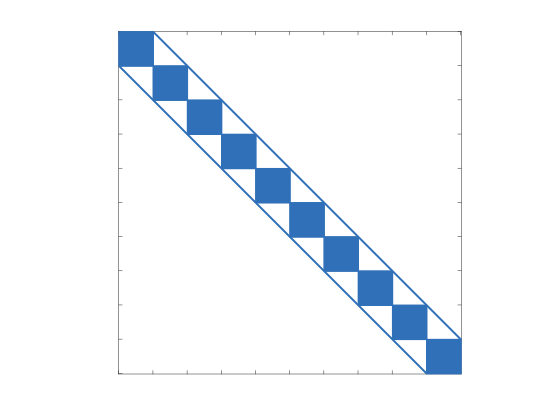
\includegraphics[width=0.5\linewidth]{Figures/tridiag_covariance.png}
    \caption{Structure of Posterior Precision Matrix, $\text{K}_{\beta}$}
    \label{fig:precision_Kbeta}
\end{figure}
%
Hence, to obtain draws from the conditional posterior of $\boldsymbol{\beta}$, we make use of the following steps:
\begin{enumerate}
    \item Compute Cholesky factor $\text{C}^{(s)}$ of $\text{K}_{\beta}^{(s)}$
    \item Generate $\text{Z}^{(s)} \sim \mvn(0,\mathbbm{I}_{\mathcal{Q} \cdot K})$
    \item Set the $\text{s}^{\text{th}}$ draw, $\boldsymbol{\beta}^{(\text{s})}$, to $\overline{\boldsymbol{\beta}}^{(s)} + ({\text{C}^{(s)}}^T)^{-1}\text{Z}^{(s)}$,
\end{enumerate}
where $\boldsymbol{\overline{\beta}^{(s)}}$ and $({\text{C}^{(s)}}^T)^{-1}$ can be found efficiently by solving linear equations. The rest of the sampling steps are standard and further explained in Appendix~\ref{app:qvp-posteriors}.
%

%To ease conditional updating of $(\nu,\lambda_{q,j})$, we represent the Cauchy distributions as a scale mixture of inverse-gamma distributed variables, as if $p(\nu) \sim C_{+}(1,A)$, then $p(\nu^2\mid \eta_{\nu}) \sim \mathrm{iG(1/2,1/\eta_{\nu})}$ and $p(\eta_{\nu}) \sim \mathrm{iG(1/2,1/A)}$ \citep{makalic2015simple}. The conditional posteriors are standard and listed in the appendix \dk{reference to the appendix}. \dk{Get rid of the $\pi$ notation for the prior probability distributions!}
%
